In PBF 3D printing processes, as with all industrial manufacturing processes, it is crucial that the process is under control, otherwise, undesirable outcomes could occur, or even the failure of the print itself. In this section, we will discuss the some defects and anomalies that can occur during PBF 3D printing. The literature review that informs the structure of this text is that of \citeauthor{mostafaei_defects_2022} (2022).
\begin{figure}
    \centering
    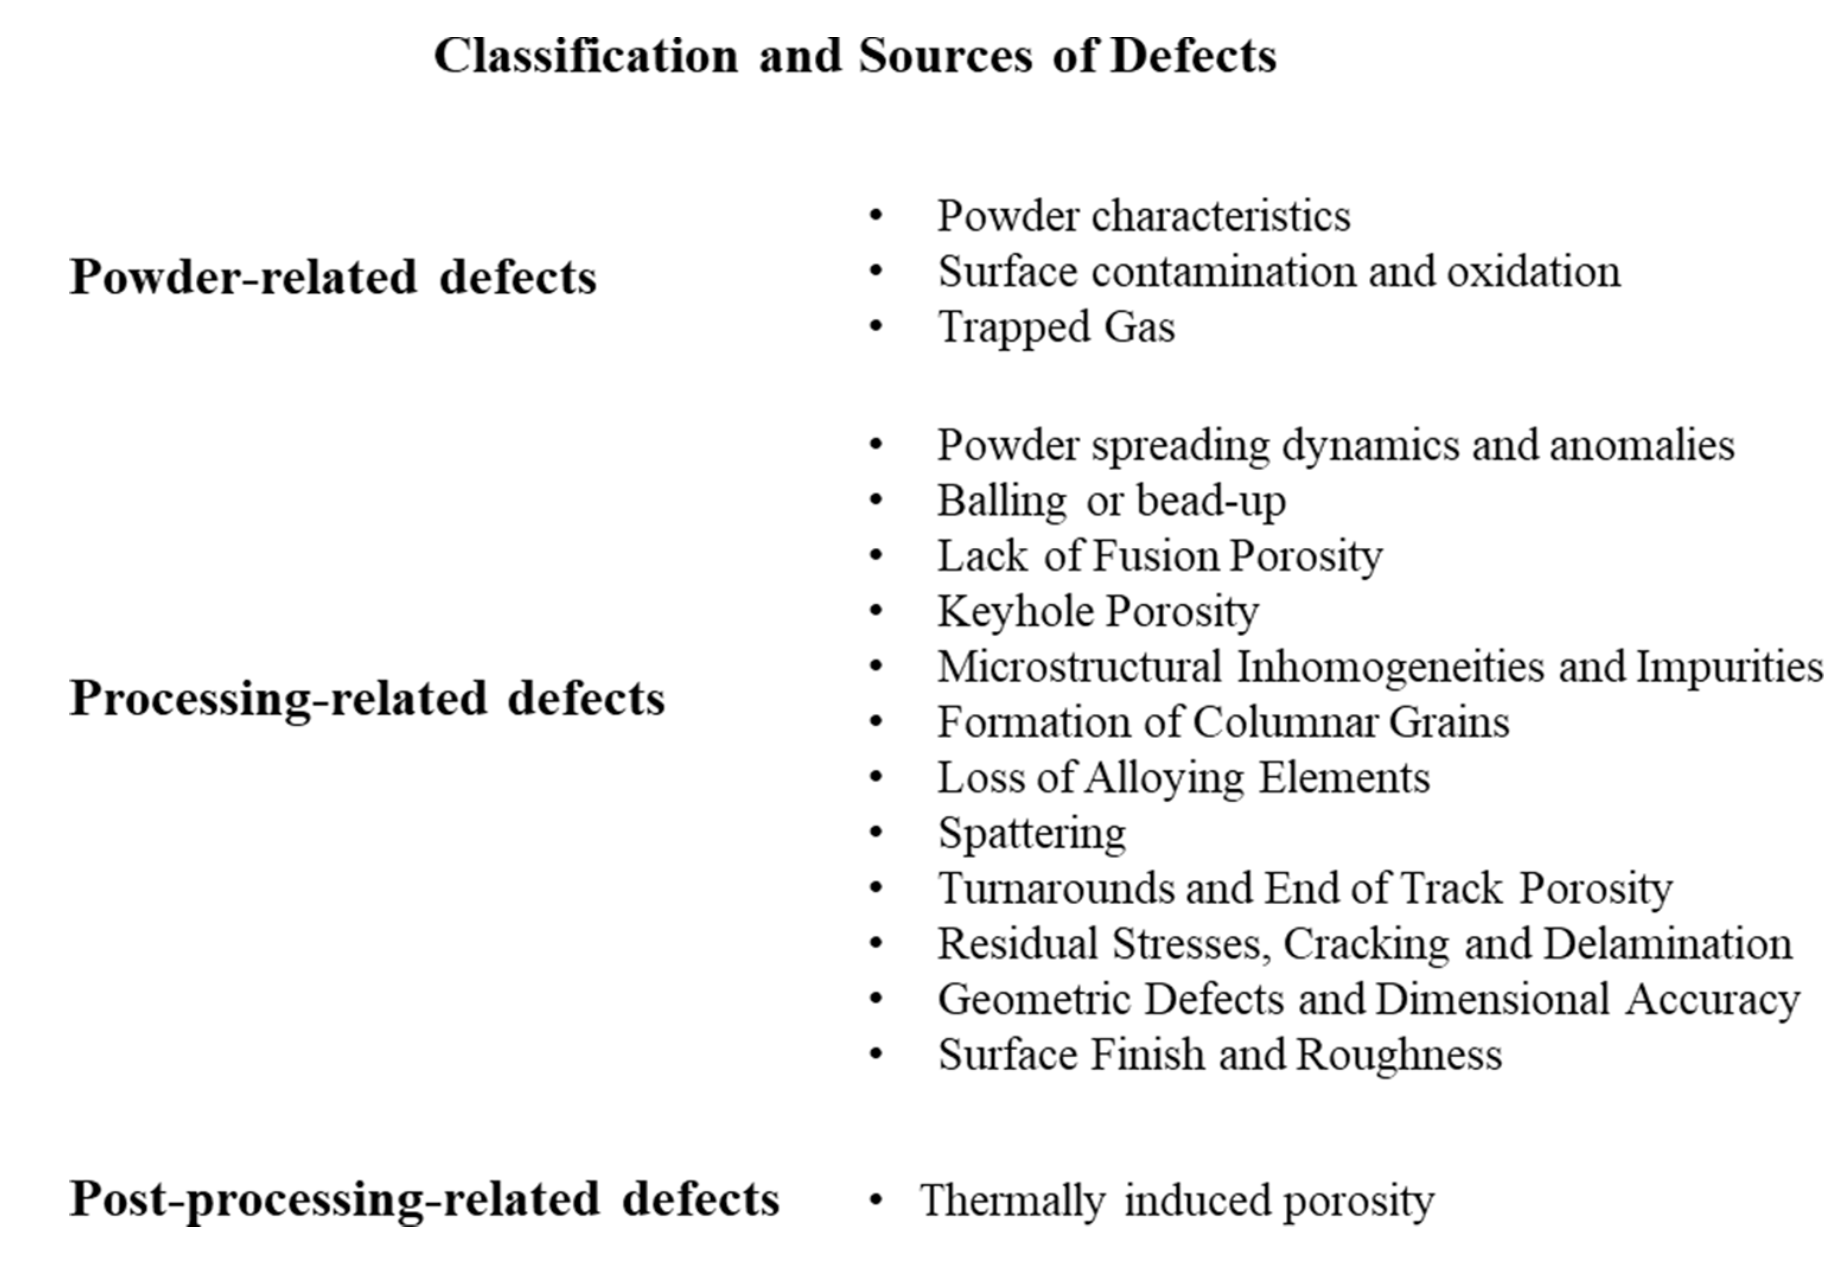
\includegraphics[width=0.7\textwidth]{Images/difettoporcodio.png}
    \caption[Defects classification in PBF.]{Defects classification in PBF processes \cite{mostafaei_defects_2022}.}
    \label{fig:difettoporcodio}
\end{figure}



\section{Hot spots}
\label{}